% !BIB TS-program = biber
\documentclass[11pt,a4paper]{article}
\usepackage[T1]{fontenc}
\usepackage[utf8]{inputenc}
\usepackage{authblk}
\usepackage{BUPTthesisbachelor}
\usepackage{setspace}
\usepackage{graphicx}

\usepackage[final]{pdfpages}

\usepackage{listings}
\usepackage{xcolor}

\usepackage{CJK}         % CJK 中文支持
\usepackage{fancyhdr}
\usepackage{amsmath,amsfonts,amssymb,graphicx}    % EPS 图片支持
\usepackage{subfigure}   % 使用子图形
\usepackage{indentfirst} % 中文段落首行缩进
\usepackage{bm}          % 公式中的粗体字符(用命令\boldsymbol)
\usepackage{multicol}    % 正文双栏

\usepackage{abstract} 

\usepackage{amssymb}
\usepackage{bm}

\usepackage{algorithm}  
\usepackage{algorithmicx}  
\usepackage{algpseudocode}  
\lstdefinestyle{sharpc}{language=[Sharp]C, frame=lrtb, rulecolor=\color{blue!80!black}}

\title{\huge{决策树ID3算法与C4.5算法研究}}

\author{席经纬}
\affil{上海交通大学\quad 电子信息与电气工程学院}


\date{}  % 这一行用来去掉默认的日期显示
%%%%%%%%%%%%%%%%%%%%%%%%% Begin Documents %%%%%%%%%%%%%%%%%%%%%%%%%%
%中文摘要
\begin{document}
\maketitle
\setlength{\oddsidemargin}{0.5cm}
\setlength{\evensidemargin}{\oddsidemargin}
\setlength{\textwidth}{14cm}
\vspace{-.8cm}
\begin{center}
\parbox{\textwidth}{
\CJKfamily{hei}摘~~~要\quad \CJKfamily{kai}~用于分类的数据挖掘技术方法有很多, 在这些方法中决策树凭借其易理解、效率高等优点而占有重要地位。ID3 算法和C4.5算法是决策树构造方法中最为常用的实现方法,它在数据分类和预测领域得到广泛应用。本文重
点总结了决策树方法中的ID3 算法和C4.5算法的研究现状, 在详细介绍ID3 和C4.5算法原理、分类依据的基础上, 比较两者的优劣。并且通过实验仿真来具体探究算法构建决策树的过程及结果。

\CJKfamily{hei}关键词\quad\CJKfamily{kai}决策树,ID3算法,C4.5算法\\}
\end{center}
\iffalse %注释
%英文摘要
\vspace{-0.5cm}
\begin{center}
\parbox{\textwidth}{
\begin{center}
\large{\textbf{Research on Development and Difficulties of Shared Economy\\——Take the example of the shared bike ofo}}
\end{center}
\vspace{-0.5cm}
\begin{center}
\textbf{Xi Jingwei}\\[2pt]
\end{center}
{\small{\textbf{Abstract}\quad 


\textbf{Key Words}\quad microbe,  artificial intelligence, computer vision,  neural network}}
}
\end{center}
\fi %注释
%%%%%%%%%%%%%%%%%%%%%%%%%%%%%%%%%%%%%%%%%%%%%%%%%%%%%%%%%%%%%%%%%%%%%
%                                                                  %
%   Copyright (c) 2010 - 2011 Caspar Zhang <casparant@gmail.com>   %
%                                                                  %
%   This copyrighted material is made available to anyone wishing  %
%   to use, modify, copy, or redistribute it subject to the terms  %
%   and conditions of the GNU General Public License version 2.    %
%                                                                  %
%   This program is distributed in the hope that it will be        %
%   useful, but WITHOUT ANY WARRANTY; without even the implied     %
%   warranty of MERCHANTABILITY or FITNESS FOR A PARTICULAR        %
%   PURPOSE. See the GNU General Public License for more details.  %
%                                                                  %
%   You should have received a copy of the GNU General Public      %
%   License along with this program; if not, write to the Free     %
%   Software Foundation, Inc., 51 Franklin Street, Fifth Floor,    %
%   Boston, MA 02110-1301, USA.                                    %
%                                                                  %
%%%%%%%%%%%%%%%%%%%%%%%%%%%%%%%%%%%%%%%%%%%%%%%%%%%%%%%%%%%%%%%%%%%%

% 你只需要修改下面几行就可以完成大部分内容的填写,
% 这要求你具有一定的LaTeX基础,但是如果你足够聪明,
% 不具有LaTeX基础也可以完成。

% 论文中文题目
\def\thesistitle{
大学生使用MOOC的影响因素研究}

\def\author{
席经纬}

    % Main ?????????????????????????????????????????items 
%%%%%%%%%%%%%%%%%%%%%%%%%%%%%%%%%%%%%%%%%%%%%%%%%%%%%%%%%%%%%%%%%%%%%
%                                                                  %
%   Copyright (c) 2010 - 2011 Caspar Zhang <casparant@gmail.com>   %
%                                                                  %
%   This copyrighted material is made available to anyone wishing  %
%   to use, modify, copy, or redistribute it subject to the terms  %
%   and conditions of the GNU General Public License version 2.    %
%                                                                  %
%   This program is distributed in the hope that it will be        %
%   useful, but WITHOUT ANY WARRANTY; without even the implied     %
%   warranty of MERCHANTABILITY or FITNESS FOR A PARTICULAR        %
%   PURPOSE. See the GNU General Public License for more details.  %
%                                                                  %
%   You should have received a copy of the GNU General Public      %
%   License along with this program; if not, write to the Free     %
%   Software Foundation, Inc., 51 Franklin Street, Fifth Floor,    %
%   Boston, MA 02110-1301, USA.                                    %
%                                                                  %
%%%%%%%%%%%%%%%%%%%%%%%%%%%%%%%%%%%%%%%%%%%%%%%%%%%%%%%%%%%%%%%%%%%%

% 你只需要修改下面内容就可以完成中英文摘要,
% 这要求你具有一定的LaTeX基础,但是还是那句话,
% 如果你足够聪明,不具有LaTeX基础也可以完成。

% 中文摘要
\def\abstractcn{
%从这里开始写你的摘要,分段需要空一行。
以MOOC为主的在线教育平台席卷全球,而当前国内外对于MOOC学习的主要群体——高校大学生的学习行为研究较少。经过
观察,大学生多是在上大学之后才开始使用MOOC,而在大学之前的学习阶段不曾使用MOOC进行学习。本文自编调查问卷,
并进行了样本特征分析、信度分析、效度检验。根据问卷调查分析
统计,文章总结出影响大学生在上大学前就开始使用MOOC的影响因素
主要有家庭经济状况、高中所在学校的性质、母亲受教育程度、父亲受教育程度。
通过对这四个影响因素的权重分析,文章指出家庭经济状况和高中学校性质
对大学生在上大学前就开始使用MOOC的影响较大。最后,文章对得出的结果进行分析,提出一些增加MOOC在中小学生群体中
使用情况的建议,以期让更多的学习者受益于优质的MOOC课程资源。


%摘要结束
}
\def\abstractcns{
随着信息技术的快速发展,教育技术也在不断变革,并给教育带来新的变化。MOOC以互联网为载体,将全球顶级大学的
优质课程资源,以极低的成本传递到原本无法取得这些资源的 世界各地学习者的终端设备上,使他们随时随地获取最优
质的学习资源。此外,MOOC学习者 可以根据时间、能力自行把握学习进度,选择学习环境,充分体现了“自主学习”的理念。

据教育部在线教育研究中心发布的《2016 中国慕课行业研究白皮书》预计,2016年中国MOOC学习者将超过 1000 万,
MOOC学习者数量呈现出快速增长趋势[。然而,尽管MOOC蓬勃发展、用户数量持续增多,但相关研究显示,MOOC的使用
者主要为高校大学生,很少的部分为中小学生。为此,本研究采用问卷调查、主成分分析等研究方法,对影响大学生在上大学前
就开始使用MOOC的影响因素进行研究,并在此基础上,提出一些增加MOOC在中小学生群体中
使用情况的建议。
}

% 中文关键字 
% TODO: 改成可变长度的
\def\abscnkeyone{MOOC}
\def\abscnkeytwo{数据分析}
\def\abscnkeythree{大学生}

  % Abstract
%%%%%%%%%%%%%%%%%%%%%%%%%%%%% Main Area %%%%%%%%%%%%%%%%%%%%%%%%%%%%
\setlength{\oddsidemargin}{-.5cm}  % 3.17cm - 1 inch
\setlength{\evensidemargin}{\oddsidemargin}
\setlength{\textwidth}{17.00cm}
\CJKfamily{song}


数据挖掘是从大量数据中发现有用知识的过程,是一种专
业技术,也是一种分析数据的手段,用于发现海量数据所隐藏
的各种规律。数据挖掘技术在对数据进行处理的过程中需要
对数据进行分类,这样才能方便之后数据的处理与预测。通常
所用到的数据分类技术是决策树分类法。决策树,顾名思义,
它是一种树形结构,包含决策节点、分支和叶节点三部分,其中决策节点代表某
个待分类数据集合的某个属性,在该属性上的不同测试结果对应一个分支,每个
叶节点表示一种可能的分类结果。

传统的决策树分类方法有ID3 和C4.5,他们都是以信息熵
作为分类依据,是单颗决策树。

\section{ID3算法}

\subsection{算法原理}
在ID3 算法中,选取信息增益最大的属性作为分类依据,然
后根据该属性的属性值构造分支。具体构造步骤如下:

step1.构造一个节点,如果所有的样本都在该节点上,那么
停止算法,将该节点改成叶子节点,并用该类标记。

step2.如果样本都不在一个节点上,求出每一个属性的信息
熵,根据公式求出每一个属性的信息增益,然后选择信息增益
最大的一个属性作为分类依据。

step3.对属性中的每一个值创建一个分支,然后划分样本。

step4.重复上述step1-step3 步骤,直到属性全部使用完。\cite{r2}

\subsection{数据划分}

ID3算法以信息熵和信息增益作为衡量标准来对样本进行分类。

\subsubsection{信息熵}
 熵的概念主要是指信息的混乱程度,变量的不确定性越大,熵的值也就越大,熵的公式可以表示为:
 
$$Entropy(S) = -\sum_{i=1}^m p(u_i)log_2p(u_i)$$
 
其中m为样本类别数,$p(u_i)$为类别在样本中出现的概率

$$p(u_i) = \frac{|u_i|}{|S|}$$

\subsubsection{信息增益}

信息增益指的是划分前后熵的变化,可以用下面的公式表示:

$$InfoGain(S, A) =Entropy(S) -\sum_{V\in Value(A)}  \frac{|S_v|}{|S|} Entropy(S_v)$$

其中,A表示样本的属性,Value(A)是属性所有的取值集合。V是A的其中一个属性值,$S_v$是S中A的值为V的样例集合。\cite{r4}


\section{C4.5算法}
\subsection{算法原理}

C4.5算法也是用于生成决策树的一种经典算法,是ID3算
法的另一种延伸和优化。C4.5算法与ID3算法生成决策树的
过程基本相同,但是ID3算法不能处理连续型属性,而C4.5算
法可以先离散化连续型属性,然后进行属性的选择分类;属性
分类时,ID3算法利用信息增益进行属性分类选择,C4.5算法则
用信息增益率进行计算。

相比于ID3 算法中,C4.5算法选取信息增益率最大的属性作为分类依据,然
后根据该属性的属性值构造分支。具体构造步骤如下:

step1.对数据预处理形成决策树训练集,如果数据是连续型属性变量,首先就应该考虑对其进行离
散化,若本身是离散值,此步省略。

step2.构造一个节点,如果所有的样本都在该节点上,那么
停止算法,将该节点改成叶子节点,并用该类标记。

step3.如果样本都不在一个节点上,求出每一个属性的信息
增益,根据公式求出每一个属性的信息增益率,然后选择信息增益率
最大的一个属性作为分类依据。

step4.对属性中的每一个值创建一个分支,然后划分样本。

step5.重复上述step2-step5 步骤,直到属性全部使用完。

\subsection{数据划分}

对于离散特征,C4.5算法不直接使用信息增益,而是使用“信息增益率”(gain ratio)\cite{r7}来选择最优的分支标准,增益率的定义如下:


$$GainRatio(S, A) = \frac{InfoGain(S, A)}{IV(A)}$$

其中IV(A)称作分支标准A的“固有值”(intrinstic value), 属性A的可能性数目越多,则IV(A)的值通常会越大。

$$IV(A) = -\sum_{V\in Value(A)}  \frac{|S_v|}{|S|} * log_2(\frac{|S_v|}{|S|})$$

\section{比较分析}

通过ID3 算法的原理及公式描述, 我们可
以发现ID3 算法是一种采用自顶向下、贪婪策略的算
法。其优势主要有以下3 点: a. 自顶向下的搜索方式
降低了搜索次数,提升了分类速度。b. ID3 算法原理清
晰,算法思路简单易懂,易于实现。c. 由于决策树在创
建的过程中都使用目前的训练样本, 而不是根据独立
的训练样本递增的做出判断, 在很大程度上降低了对
个别训练样本错误的敏感性 。\cite{r1}ID3 算法不足主要有以
下四点:a. ID3 算法对噪声数据相对敏感, 算法依赖于属性值数目较多的属
性,但是属性值较多的属性不一定是分类最优的属性。 b.  ID3 算法
循环调用过程中会产生大量的对数运算, 随着样本集
合、属性以及属性取值个数的增加, 对数运算次数将
会大大增加,从而降低了ID3 算法的运算效率,产生了
极大的时间开销。c. ID3 算法在建树过程中不进行回
溯导致生成的决策树节点只是局部最优的, 相对于全
局, 往往不是我们所期待的结果, 即如多值偏向所得
结果并不总是最优结果。d. ID3 只能分类离散型数据。\cite{r6}

C4.5算法继承了ID3 算法的优点,并在以下几方面对ID3 算法进行了改进\cite{r5}:
a. 用信息增益率来选择属性,克服了用信息增益选择属性
时偏向选择取值多的属性的不足。
b. 在树构造过程中进行剪枝。
c. 能够完成对连续属性的离散化处理。
d. 能够对不完整数据进行处理。
这样,C4.5算法构造树的准确率更高,产生的分类
规则更容易理解,以信息增益率选择分裂属性克服ID3的缺点,并
能把连续型的属性变量离散化。同时,在构造决策树过程中,能够对缺失
属性值的进行处理,采用后剪枝技术等。\cite{r3}


\section{实验仿真}

选取UCI隐形眼镜数据集,通过ID3算法与C4.5算法构建决策树来根据患者的年龄(age)、症状(prescript)、是否散光(astigmatic)、眼泪数量(tearRate)等属性推荐隐形眼镜类型。

\subsection{实验数据集}

实验采用UCI隐形眼镜数据集,它包含很多患者眼部状态的观察属性以及医生推荐的隐形眼镜类型。隐形眼镜类型包括硬材质(hard)、软材质(soft)以及不适合佩戴隐形眼镜(no lenses)。

数据集每一行数据的Labels依次是序号(ID)、年龄(age)、症状(prescript)、是否散光(astigmatic)、眼泪数量(tearRate)、分类(class)。训练数据集有100组数据,测试数据集有24组数据。

标签属性:

    1. age of the patient: (1) young, (2) pre-presbyopic, (3) presbyopic
    
    2. spectacle prescription:  (1) myope, (2) hypermetrope
    
    3. astigmatic:     (1) no, (2) yes
    
    4. tear production rate:  (1) reduced, (2) normal
    

\subsection{实验结果}

根据上面描述的算法,我们构建出隐形眼镜决策树:

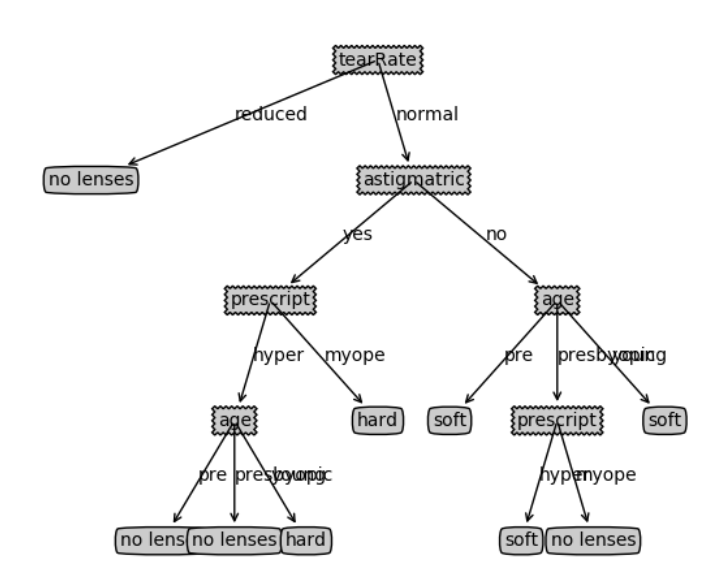
\includegraphics[scale=0.5]{abc.png}

ID3算法在训练数据集上可以达到94\%的准确率,在测试数据集上准确率为91.6667\%,C4.5算法在训练数据集上可以达到94\%的准确率,在测试数据集上准确率为91.6667\%


\section{总结与展望}

作为决策树中经典算法,ID3 算法使用
信息增益作为分类标准, 凭借其分类速度快、实现方
式简单等优点, 成为了具有适用与研究价值的示例学
习算法与知识获取的有效工具。C4.5算法在ID3算法的基础上进行改进,提高了准确率。
目前,决策树分类算法应用领域十分广泛
, 如医学中的病症分类预测和基因与高分子序列分
析、商业活动中的市场分析和人力资源管理、教育行
业中的成绩分析、高校管理等。同时,研究者们也在不
断对决策树分类算法进行优化与改进,提升了分类效率,获得
了更好的分类结果。在当前大数据技术背景下, 会有
更多改进算法被提出,决策树算法也会在更多的领域
得到应用。






%%%%%%%%%%%%%%%%%%%%%%% Main Area ENDs Here %%%%%%%%%%%%%%%%%%%%%%%%
\addcontentsline{toc}{chapter}{参考文献}
\begin{thebibliography}{00}
  \bibitem{r1} 徐梦茹,王学明.决策树几种分类算法的分析比较.《电脑知识与技术》, 2018.07
  \bibitem{r2} 曹颖超.决策树分类算法及其应用 《信息技术》,2018.01
  \bibitem{r3} 马俊宏. 数据挖掘技术决策树分类算法分析、比较与实验. 《北京印刷学院学报》, 2017.11
   \bibitem{r4}杜威铭,冉羽 .决策树ID3 算法研究.《科技视界》, 2018.11
   \bibitem{r5}张宏,高长松. C4.5 算法对ID3算法的改进 . 《计算机光盘软件与应用》,2012.06
    \bibitem{r6}刘瑞玲. C4.5 决策树分类算法性能分析 . 《信息系统工程》,2014.05
    \bibitem{r7}王文霞. 数据挖掘中改进的C4.5决策树分类算法 . 《吉林大学学报》,2017.09
\end{thebibliography}

\end{document}